\documentclass[twoside,UTF8]{EPURapport}
%\usepackage{listings}

%\renewcommand{\lstlistlistingname}{Liste des codes}
%\renewcommand{\lstlistingname}{Code}

%\addextratables{%
%	\lstlistoflistings
%}

%\swapAuthorsAndSupervisors
\nolistoffigures
\nolistoftables


\usepackage{amsmath}
\usepackage{amsfonts}
\usepackage{amssymb}

\usepackage{float}
%\usepackage{color}
\usepackage{array}
\usepackage{multirow}
%\usepackage{xcolor}
\usepackage{supertabular}
\usepackage{longtable}
\usepackage{algorithmic}
\usepackage{algorithm}
\usepackage{hyperref}

\usepackage{graphicx}
\usepackage{caption}
\usepackage{subcaption}


\renewcommand{\algorithmicrequire}{\textbf{Entrées et pr\'{e}condition:}}
\renewcommand{\algorithmicensure}{\textbf{Sorties et postcondition:}}
\renewcommand{\algorithmicend}{\textbf{fin}}
\renewcommand{\algorithmicif}{\textbf{si}}
\renewcommand{\algorithmicthen}{\textbf{alors}}
\renewcommand{\algorithmicelse}{\textbf{sinon}}
\renewcommand{\algorithmicelsif}{\algorithmicelse\ \algorithmicif} 
\renewcommand{\algorithmicendif}{\algorithmicend\ \algorithmicif} 
\renewcommand{\algorithmicfor}{\textbf{pour}}
\renewcommand{\algorithmicforall}{\textbf{pour tout}} 
\renewcommand{\algorithmicdo}{\textbf{faire}}
\renewcommand{\algorithmicendfor}{\algorithmicend\ \algorithmicfor} 
\renewcommand{\algorithmicwhile}{\textbf{tant que}}
\renewcommand{\algorithmicendwhile}{\algorithmicend\ \algorithmicwhile} 
\renewcommand{\algorithmicloop}{\textbf{boucle}}
\renewcommand{\algorithmicendloop}{\algorithmicend\ \algorithmicloop} 
\renewcommand{\algorithmicrepeat}{\textbf{répéter}}
\renewcommand{\algorithmicuntil}{\textbf{jusqu'à}}
\renewcommand{\algorithmictrue}{\textbf{vrai}}
\renewcommand{\algorithmicfalse}{\textbf{faux}}
\renewcommand{\algorithmiccomment}[1]{$/*$~#1~$*/$}
\floatname{algorithm}{Algorithme}
\renewcommand{\listalgorithmname}{Liste des algorithmes}

\thedocument{Manipulation des détails d'une image}{Développement d’un outil de traitement d’images par filtrage bilatéral}{Décomposition pyramidale du filtre bilatéral}

\grade{Département Informatique\\ 5\ieme{} année\\ 2014 - 2015}

\authors{%
	\category{Étudiants}{%
		\name{Natacha \textsc{Marlio-Ma}} \mail{natacha.marlio-marette@etu.univ-tours.fr}
	}
	\details{DI5 2014 - 2015}
}

\supervisors{%
	\category{Encadrants}{%
		\name{Moncef \textsc{Hidane}} \mail{moncef.hidane@insa-cvl.fr}
	}
	\details{INSA, Blois}
}

\abstracts{}
{}
{}
{}

\begin{document}

\chapter{Introduction}

\paragraph{}
La décomposition pyramidale permet d'obtenir un ensemble d'images composés des couches de bases (\textit{u}) et détails (\textit{d}) qui avec l'équation \ref{eq:imgOri} permet de reconstituer l'image originale. 

\begin{equation}
\label{eq:imgOri}
	g = b + \sum^{k}_{i=1}d^{i}
\end{equation}

\paragraph{}
Soit $d^i$ (respectivement $u^i$) la couche de détail (respectivement la couche de base) obtenue à l'itération \textit{i} et \textit{b} la dernière couche de base de l'itération \textit{k}. Soit \textit{g} l'image reconstruite.

\paragraph{}
Afin de manipuler le niveau de détails de l'image, l'équation \ref{eq:imgOri} va être légèrement modifiée. Les différentes couches de détails \textit{d} et la couche de base \textit{b} seront multiplié par un coefficient $\beta$ et $\alpha$ ce qui donnera l'équation \ref{eq:manipDetail}. 
\begin{equation}
\label{eq:manipDetail}
	g = \alpha*b + \sum^{k}_{i=1}\beta*(i+1)*d^{i} 
\end{equation}

\paragraph{}
Les méthodes misent en place sont celles décrites dans le document sur la décomposition pyramidale du filtre bilatéral. 

\chapter{Manipulation des détails : Atténuation}

\paragraph{}
Après des tests des différentes valeurs de $\alpha$ et $\beta$ présent dans l'équation \ref{eq:manipDetail} afin de trouver leur valeur optimale dans le but d'atténuer les détails de l'image. 

\begin{figure}[H]
        \centering
        \begin{subfigure}[b]{0.3\textwidth}
                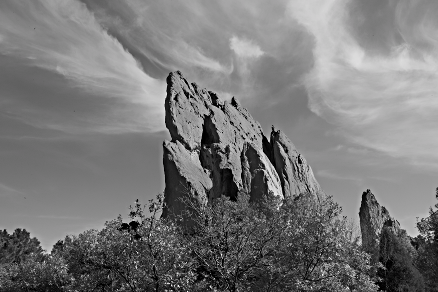
\includegraphics[scale=0.4]{images/rock_input1_1_08.png} 
                \caption{Méthode 1}
        \end{subfigure}
        \qquad \qquad
        \begin{subfigure}[b]{0.3\textwidth}
                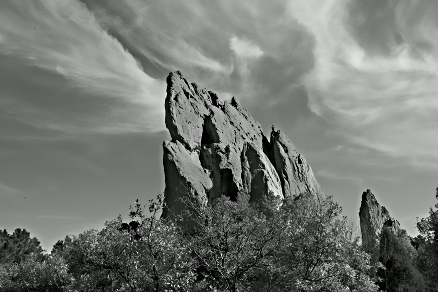
\includegraphics[scale=0.4]{images/rock_input2_1_08.png}
                \caption{Méthode 2}
        \end{subfigure}
        
        \begin{subfigure}[b]{0.3\textwidth}
                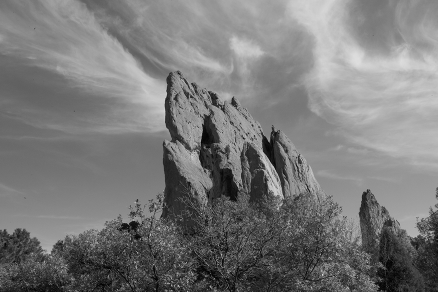
\includegraphics[scale=0.4]{images/rock_input.png}
             	\caption{Image originale}
        \end{subfigure}
        \caption{Atténuation des détails avec $\alpha$=1 et $\beta$=0.8}
\end{figure}


\begin{figure}
        \centering
        \begin{subfigure}[b]{0.3\textwidth}
                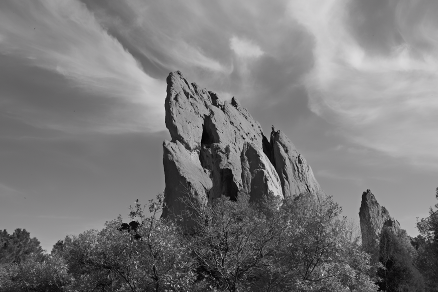
\includegraphics[scale=0.4]{images/rock_input1_1_05.png} 
                \caption{Méthode 1}
        \end{subfigure}
        \qquad \qquad
        \begin{subfigure}[b]{0.3\textwidth}
                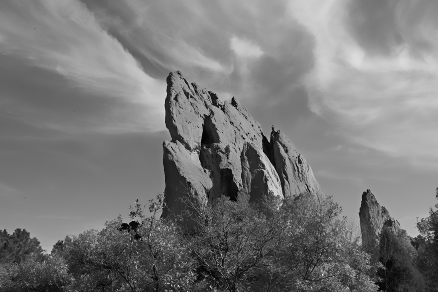
\includegraphics[scale=0.4]{images/rock_input2_1_05.png}
                \caption{Méthode 2}
        \end{subfigure}
        
        \begin{subfigure}[b]{0.3\textwidth}
                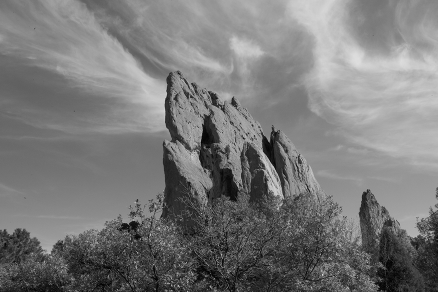
\includegraphics[scale=0.4]{images/rock_input.png}
             	\caption{Image originale}
        \end{subfigure}
        \caption{Atténuation des détails avec $\alpha$=1 et $\beta$=0.5}
\end{figure}

\begin{figure}
        \centering
        \begin{subfigure}[b]{0.3\textwidth}
                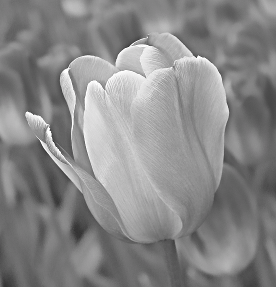
\includegraphics[scale=0.45]{images/flower1_1_08.png} 
                \caption{Méthode 1}
        \end{subfigure}
        \qquad \qquad
        \begin{subfigure}[b]{0.3\textwidth}
                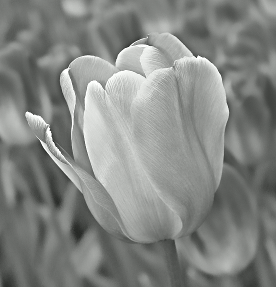
\includegraphics[scale=0.45]{images/flower2_1_08.png}
                \caption{Méthode 2}
        \end{subfigure}
        
        \begin{subfigure}[b]{0.3\textwidth}
                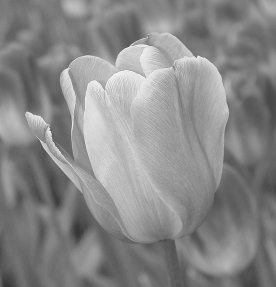
\includegraphics[scale=0.45]{images/flower.png}
             	\caption{Image originale}
        \end{subfigure}
        \caption{Atténuation des détails avec $\alpha$=1 et $\beta$=0.8}
\end{figure}

\begin{figure}
        \centering
        \begin{subfigure}[b]{0.3\textwidth}
                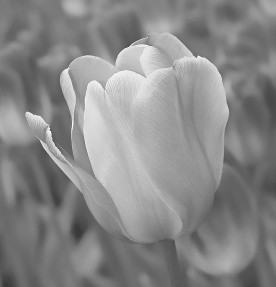
\includegraphics[scale=0.45]{images/flower1_1_05.png} 
                \caption{Méthode 1}
        \end{subfigure}
        \qquad \qquad
        \begin{subfigure}[b]{0.3\textwidth}
                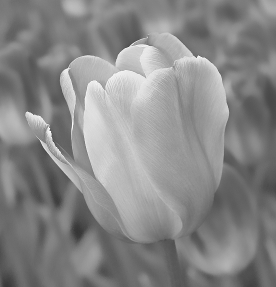
\includegraphics[scale=0.45]{images/flower2_1_05.png}
                \caption{Méthode 2}
        \end{subfigure}
        
        \begin{subfigure}[b]{0.3\textwidth}
                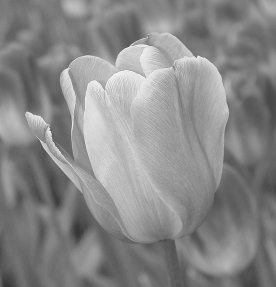
\includegraphics[scale=0.45]{images/flower.png}
             	\caption{Image originale}
        \end{subfigure}
        \caption{Atténuation des détails avec $\alpha$=1 et $\beta$=0.5}
\end{figure}

\begin{figure}
        \centering
        \begin{subfigure}[b]{0.3\textwidth}
                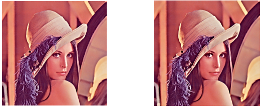
\includegraphics[]{images/lena1_08.png} 
                \caption{Méthode 1 et 2}
        \end{subfigure}
        
        \begin{subfigure}[b]{0.3\textwidth}
                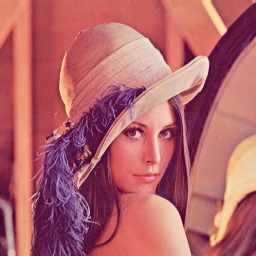
\includegraphics[scale=0.5]{images/lena.jpg}
             	\caption{Image originale}
        \end{subfigure}
        \caption{Atténuation des détails avec $\alpha$=1 et $\beta$=0.8}
\end{figure}

\begin{figure}
        \centering
        \begin{subfigure}[b]{0.3\textwidth}
                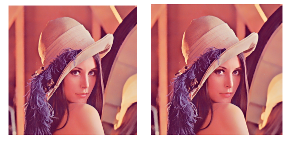
\includegraphics[]{images/lena_1_05.png} 
                \caption{Méthode 1 et 2}
        \end{subfigure}
        
        \begin{subfigure}[b]{0.3\textwidth}
                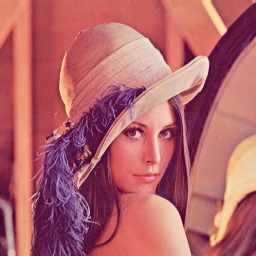
\includegraphics[scale=0.5]{images/lena.jpg}
             	\caption{Image originale}
        \end{subfigure}
        \caption{Atténuation des détails avec $\alpha$=1 et $\beta$=0.5}
\end{figure}

\chapter{Manipulation des détails : Réhaussement}

\paragraph{}
La recherche des valeurs de $\alpha$ et $\beta$ de l'équation \ref{eq:manipDetail} est réitérée afin d'obtenir les paramètres permettant de réhausser au mieux le niveau de détail de l'image. 

\begin{figure}[H]
        \centering
        \begin{subfigure}[b]{0.3\textwidth}
                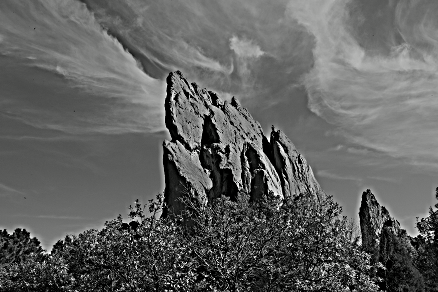
\includegraphics[scale=0.4]{images/rock_input1_08_1.png} 
                \caption{Méthode 1}
        \end{subfigure}
        \qquad \qquad
        \begin{subfigure}[b]{0.3\textwidth}
                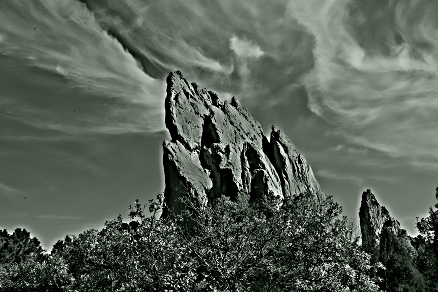
\includegraphics[scale=0.4]{images/rock_input2_08_1.png}
                \caption{Méthode 2}
        \end{subfigure}
        
        \begin{subfigure}[b]{0.3\textwidth}
                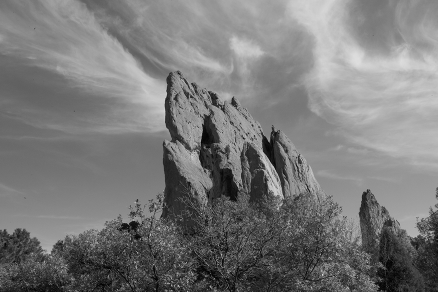
\includegraphics[scale=0.4]{images/rock_input.png}
             	\caption{Image originale}
        \end{subfigure}
        \caption{Réhaussement des détails avec $\alpha$=0.8 et $\beta$=1 }
\end{figure}

\begin{figure}
        \centering
        \begin{subfigure}[b]{0.3\textwidth}
                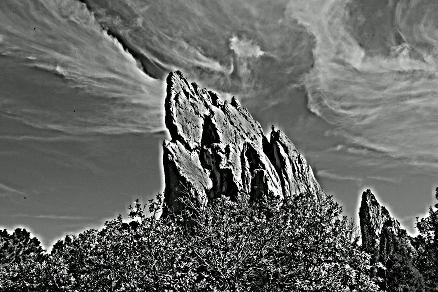
\includegraphics[scale=0.4]{images/rock_input1_08_3.png} 
                \caption{Méthode 1}
        \end{subfigure}
        \qquad \qquad
        \begin{subfigure}[b]{0.3\textwidth}
                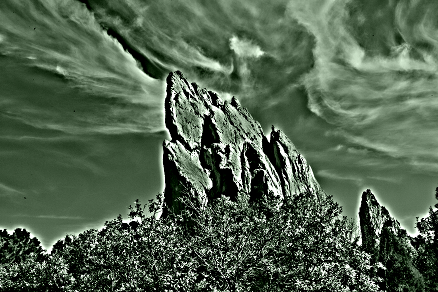
\includegraphics[scale=0.4]{images/rock_input2_08_3.png}
                \caption{Méthode 2}
        \end{subfigure}
        
        \begin{subfigure}[b]{0.3\textwidth}
                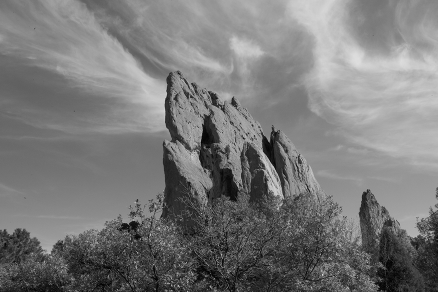
\includegraphics[scale=0.4]{images/rock_input.png}
             	\caption{Image originale}
        \end{subfigure}
        \caption{Réhaussement des détails avec $\alpha$=0.8 et $\beta$=3 }
\end{figure}

\begin{figure}
        \centering
        \begin{subfigure}[b]{0.3\textwidth}
                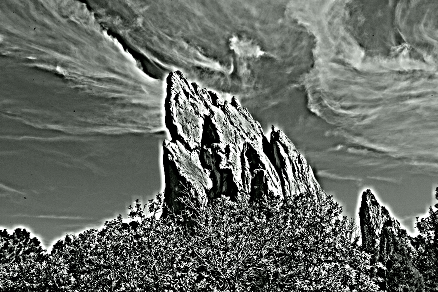
\includegraphics[scale=0.4]{images/rock_input1_08_5.png} 
                \caption{Méthode 1}
        \end{subfigure}
        \qquad \qquad
        \begin{subfigure}[b]{0.3\textwidth}
                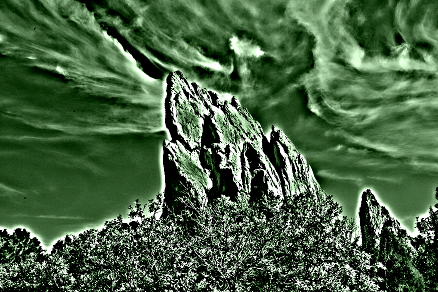
\includegraphics[scale=0.4]{images/rock_input2_08_5.png}
                \caption{Méthode 2}
        \end{subfigure}
        
        \begin{subfigure}[b]{0.3\textwidth}
                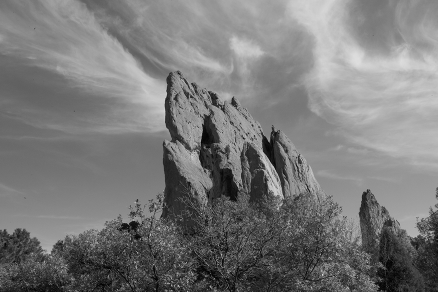
\includegraphics[scale=0.4]{images/rock_input.png}
             	\caption{Image originale}
        \end{subfigure}
        \caption{Réhaussement des détails avec $\alpha$=0.8 et $\beta$=5 }
\end{figure}

\begin{figure}[H]
        \centering
        \begin{subfigure}[b]{0.3\textwidth}
                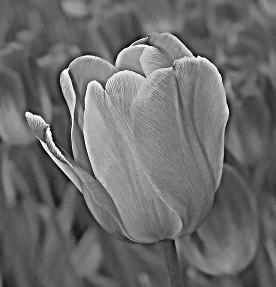
\includegraphics[scale=0.45]{images/flower1_08_1.png} 
                \caption{Méthode 1}
        \end{subfigure}
        \qquad \qquad
        \begin{subfigure}[b]{0.3\textwidth}
                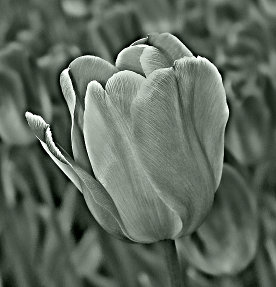
\includegraphics[scale=0.45]{images/flower2_08_1.png}
                \caption{Méthode 2}
        \end{subfigure}
        
        \begin{subfigure}[b]{0.3\textwidth}
                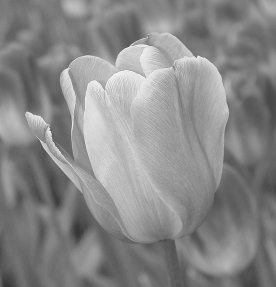
\includegraphics[scale=0.45]{images/flower.png}
             	\caption{Image originale}
        \end{subfigure}
        \caption{Réhaussement des détails avec $\alpha$=0.8 et $\beta$=1 }
\end{figure}

\begin{figure}[H]
        \centering
        \begin{subfigure}[b]{0.3\textwidth}
                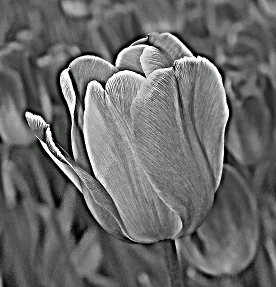
\includegraphics[scale=0.45]{images/flower1_08_3.png} 
                \caption{Méthode 1}
        \end{subfigure}
        \qquad \qquad
        \begin{subfigure}[b]{0.3\textwidth}
                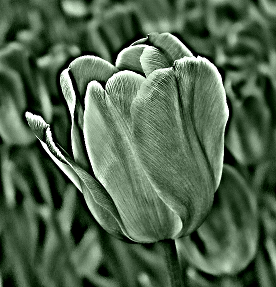
\includegraphics[scale=0.45]{images/flower2_08_3.png}
                \caption{Méthode 2}
        \end{subfigure}
        
        \begin{subfigure}[b]{0.3\textwidth}
                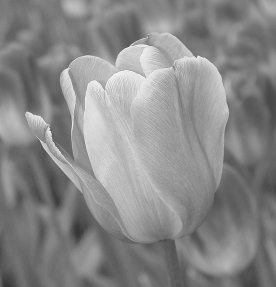
\includegraphics[scale=0.45]{images/flower.png}
             	\caption{Image originale}
        \end{subfigure}
        \caption{Réhaussement des détails avec $\alpha$=0.8 et $\beta$=3 }
\end{figure}

\begin{figure}[H]
        \centering
        \begin{subfigure}[b]{0.3\textwidth}
                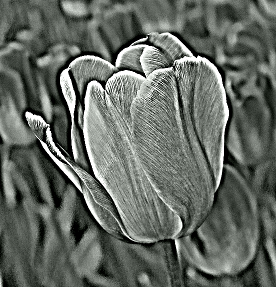
\includegraphics[scale=0.45]{images/flower1_08_5.png} 
                \caption{Méthode 1}
        \end{subfigure}
        \qquad \qquad
        \begin{subfigure}[b]{0.3\textwidth}
                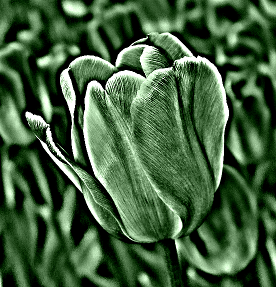
\includegraphics[scale=0.45]{images/flower2_08_5.png}
                \caption{Méthode 2}
        \end{subfigure}
        
        \begin{subfigure}[b]{0.3\textwidth}
                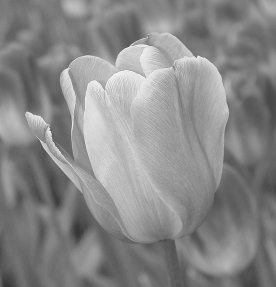
\includegraphics[scale=0.45]{images/flower.png}
             	\caption{Image originale}
        \end{subfigure}
        \caption{Réhaussement des détails avec $\alpha$=0.8 et $\beta$=5}
\end{figure}

\begin{figure}[H]
        \centering
        \begin{subfigure}[b]{0.3\textwidth}
                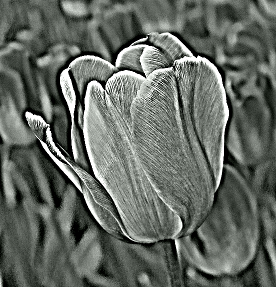
\includegraphics[scale=0.45]{images/flower1_08_5.png} 
                \caption{Méthode 1}
        \end{subfigure}
        \qquad \qquad
        \begin{subfigure}[b]{0.3\textwidth}
                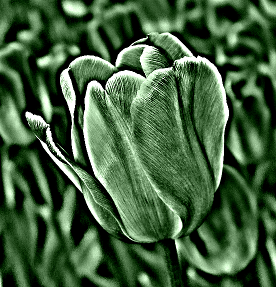
\includegraphics[scale=0.45]{images/flower2_08_5.png}
                \caption{Méthode 2}
        \end{subfigure}
        
        \begin{subfigure}[b]{0.3\textwidth}
                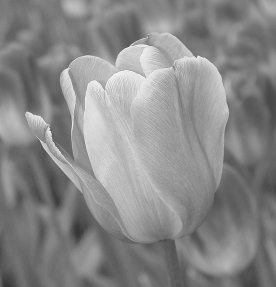
\includegraphics[scale=0.45]{images/flower.png}
             	\caption{Image originale}
        \end{subfigure}
        \caption{Réhaussement des détails avec $\alpha$=0.8 et $\beta$=5}
\end{figure}

\begin{figure}
	\centering
        \begin{subfigure}[b]{0.3\textwidth}
                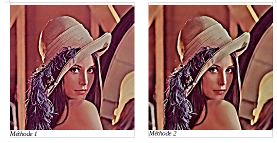
\includegraphics[]{images/lena_08_1.png}
                \caption{Méthode 1 et 2}
        \end{subfigure}
        
        \begin{subfigure}[b]{0.3\textwidth}
                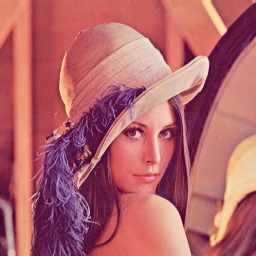
\includegraphics[scale=0.5]{images/lena.jpg}
             	\caption{Image originale}
        \end{subfigure}
        \caption{Réhaussement des détails avec $\alpha$=0.8 et $\beta$=1}
\end{figure}

\begin{figure}
        \centering
        \begin{subfigure}[b]{0.3\textwidth}
                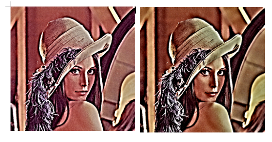
\includegraphics[]{images/lena_08_3.png} 
                \caption{Méthode 1 et 2}
        \end{subfigure}
        
        \begin{subfigure}[b]{0.3\textwidth}
                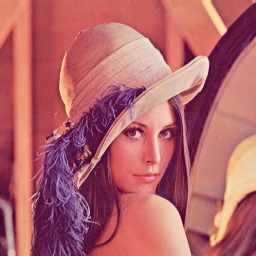
\includegraphics[scale=0.5]{images/lena.jpg}
             	\caption{Image originale}
        \end{subfigure}
        \caption{Réhaussement des détails avec $\alpha$=0.8 et $\beta$=3}
\end{figure}

\begin{figure}
        \centering
        \begin{subfigure}[b]{0.3\textwidth}
                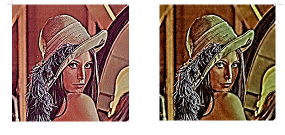
\includegraphics[]{images/lena_08_5.png} 
                \caption{Méthode 1 et 2}
        \end{subfigure}
        
        \begin{subfigure}[b]{0.3\textwidth}
                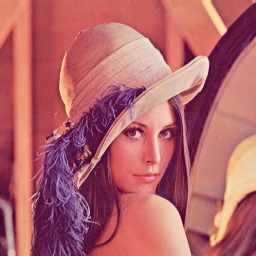
\includegraphics[scale=0.5]{images/lena.jpg}
             	\caption{Image originale}
        \end{subfigure}
        \caption{Réhaussement des détails avec $\alpha$=0.8 et $\beta$=5}
\end{figure}

%\bibliography{biblio}
%\bibliographystyle{unsrt}
%\addcontentsline{toc}{chapter}{Bibliographie}

\end{document}